\chapter{Grundlagen}
\section{Abgrenzung zu VR im Rahmen des Moduls}
\section{A* Algorithmus}
Der A*-Algorithmus ist ein Wegfindungs-Algorithmus, der von Peter Hart, Nils Nilsson und
Bertram Raphael entwickelt wurde. Sein Ziel ist es den schnellsten Weg in einem Grafen vom Startknoten zum Zielknoten zu finden. 
\subsection{Funktionsweise}
Der Ausgangspunkt bildet ein zwei-dimensionales Array in dem es Felder gibt, die entweder Pfad und Hindernis darstellen. Es wird ein Start- sowie Zielfeld festgelegt. Beide sind dem Algorithmus während der Ausführung bekannt.Sobald das Spielfeld erstellt sowie ein Start- und Zielfeld gewählt wurde, sind die Mindestvoraussetzungen erfüllt.

\begin{figure}
    \centering
    \begin{subfigure}[b]{0.3\textwidth}
        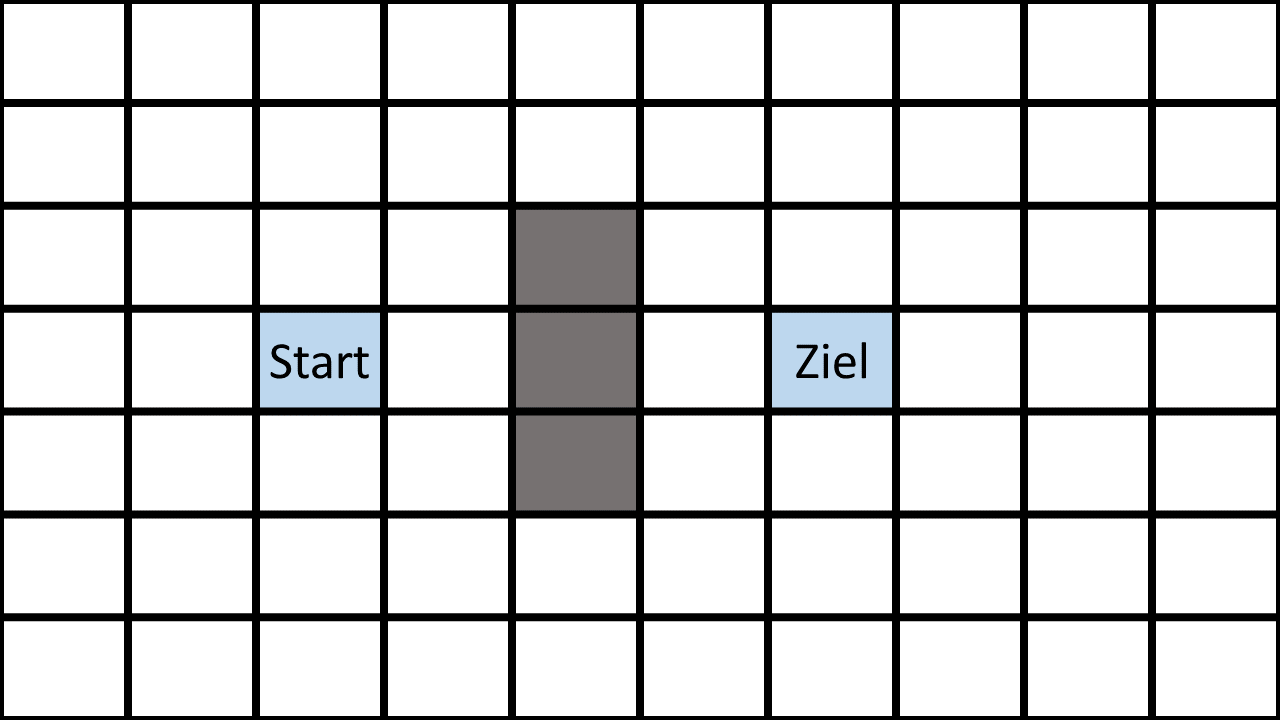
\includegraphics[width=\textwidth]{assets/aStarStep0.png}
        \caption{Schritt 1}
        \label{fig:aStartStep1}
    \end{subfigure}
    ~ %add desired spacing between images, e. g. ~, \quad, \qquad, \hfill etc. 
    %(or a blank line to force the subfigure onto a new line)
    \begin{subfigure}[b]{0.3\textwidth}
        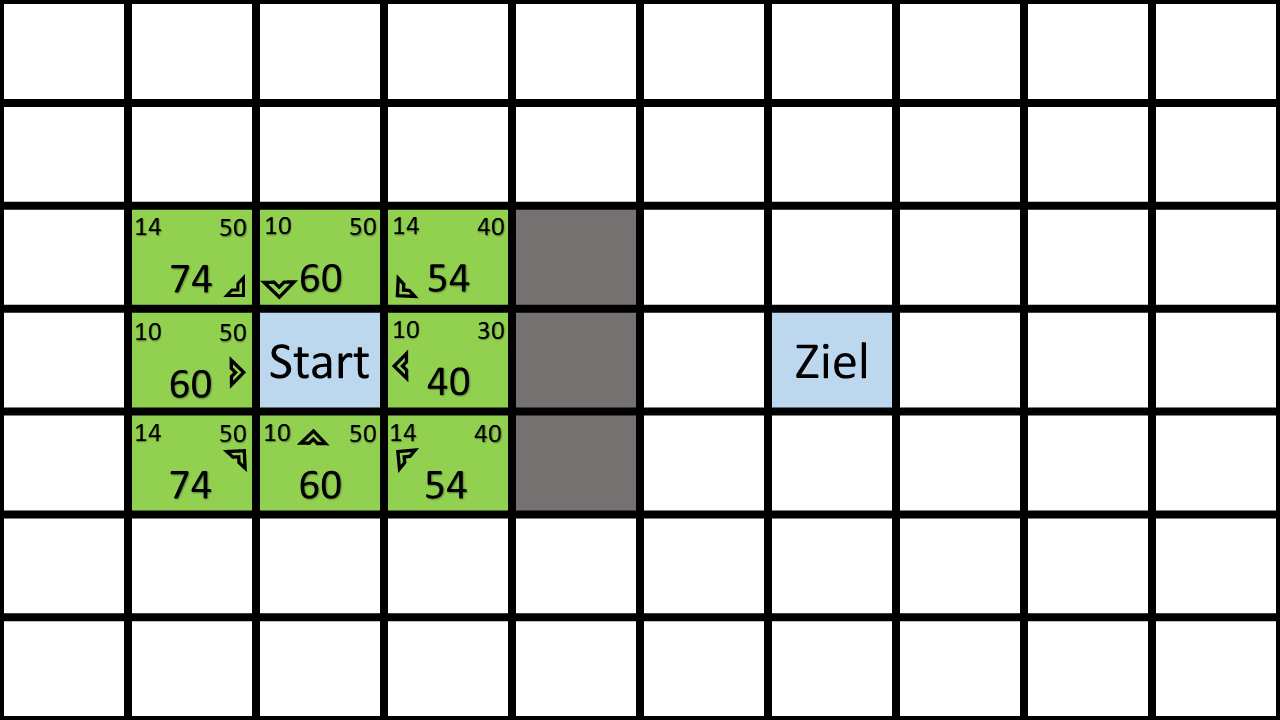
\includegraphics[width=\textwidth]{assets/aStarStep1.png}
        \caption{Schritt 2}
        \label{fig:aStartStep2}
    \end{subfigure}
    ~
    \begin{subfigure}[b]{0.3\textwidth}
        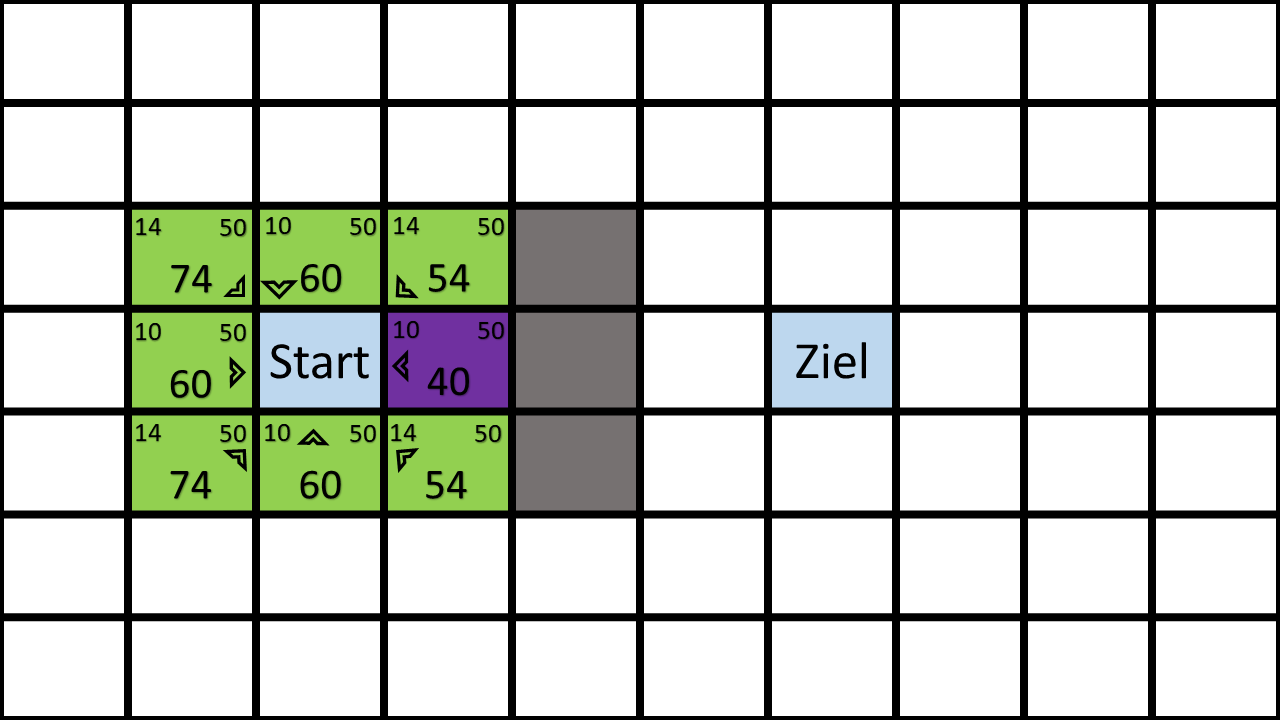
\includegraphics[width=\textwidth]{assets/aStarStep2.png}
        \caption{Schritt 3}
        \label{fig:aStartStep3}
    \end{subfigure}
    \caption{A* Ausführungsschritte 1-3}\label{fig:aStarStep1_3}
\end{figure}


\begin{figure}
    \centering
    \begin{subfigure}[b]{0.3\textwidth}
        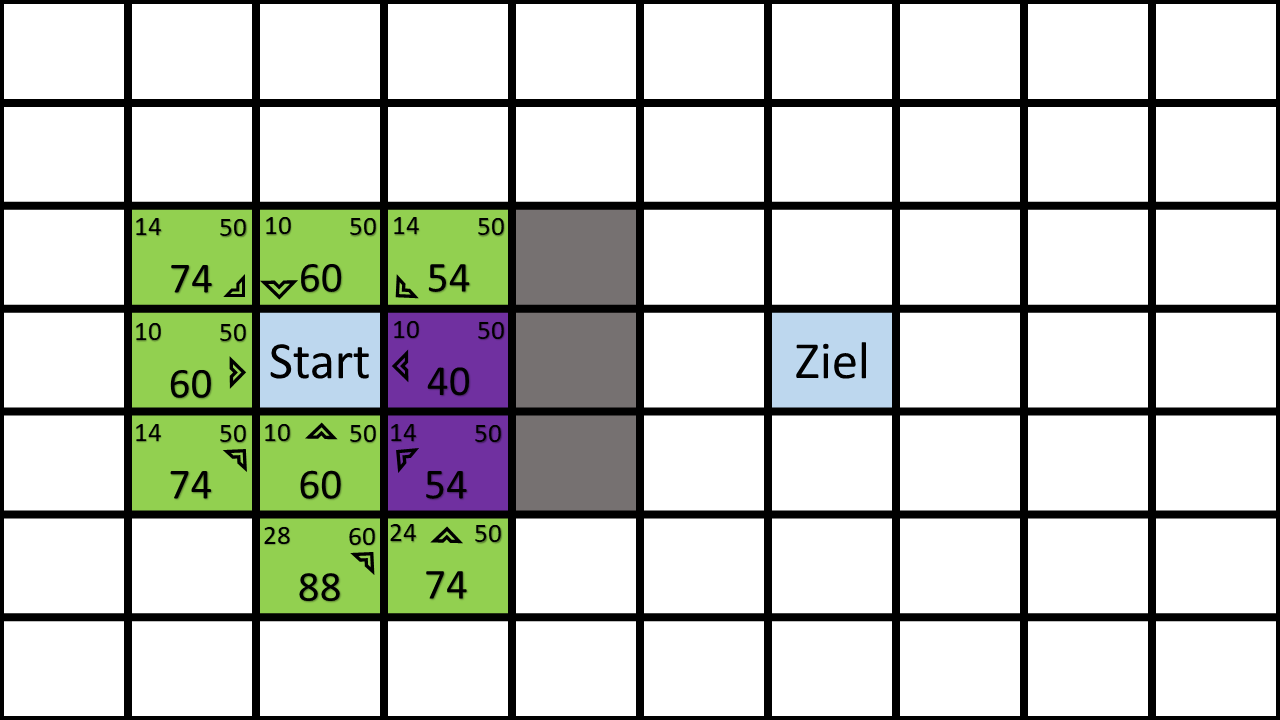
\includegraphics[width=\textwidth]{assets/aStarStep3.png}
        \caption{Schritt 4}
        \label{fig:aStartStep4}
    \end{subfigure}
    ~
    \begin{subfigure}[b]{0.3\textwidth}
        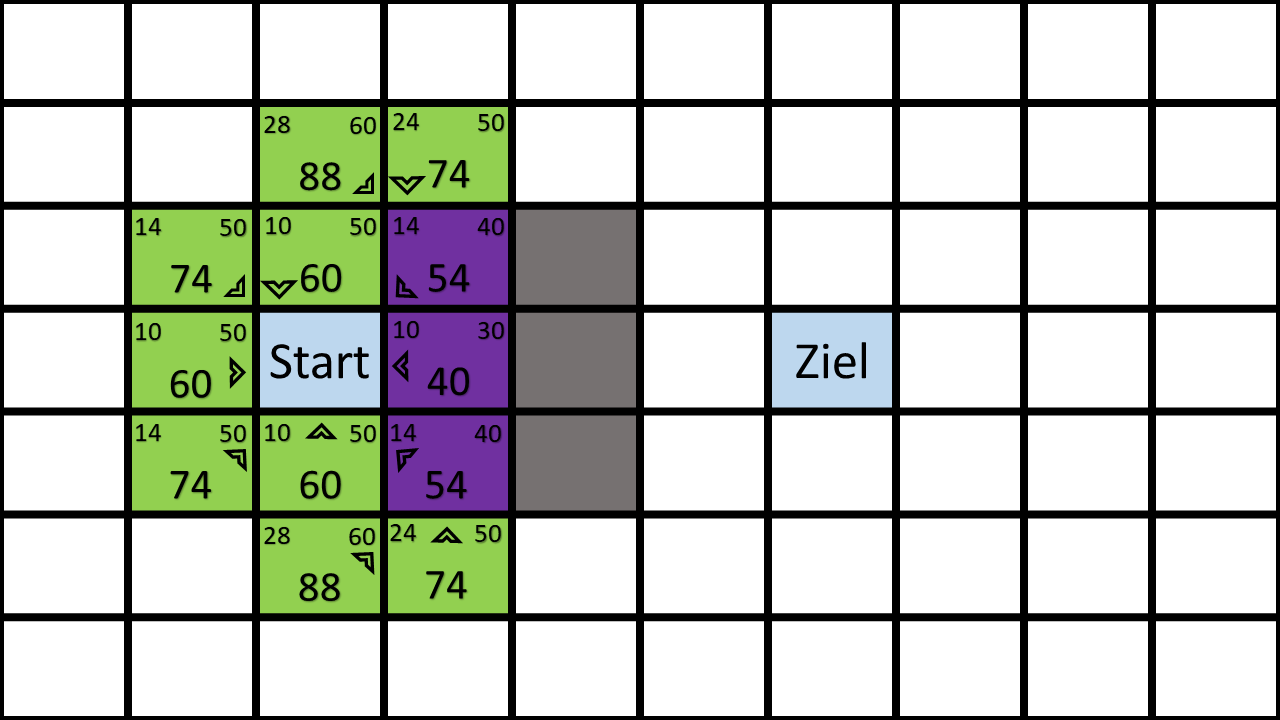
\includegraphics[width=\textwidth]{assets/aStarStep4.png}
        \caption{Schritt 5}
        \label{fig:aStartStep5}
    \end{subfigure}
    ~
    \begin{subfigure}[b]{0.3\textwidth}
        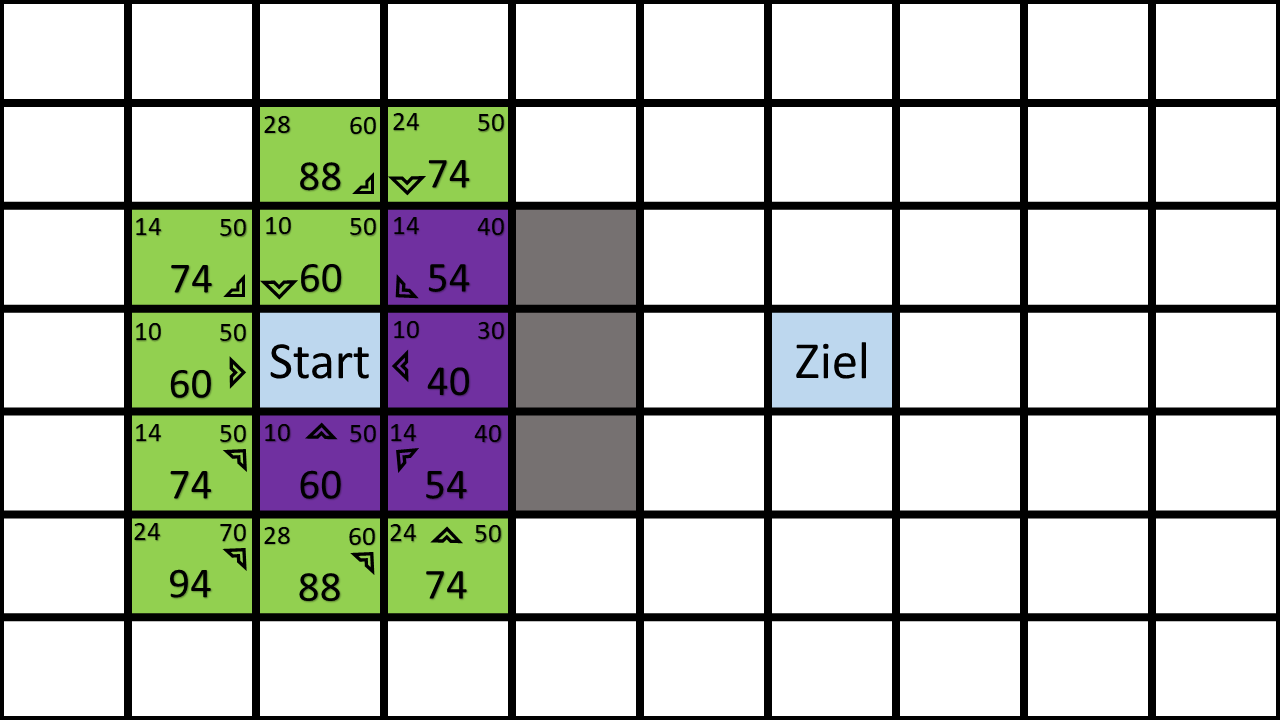
\includegraphics[width=\textwidth]{assets/aStarStep5.png}
        \caption{Schritt 6}
        \label{fig:aStartStep6}
    \end{subfigure}
    \caption{A* Ausführungsschritte 4-6}\label{fig:aStarStep4_6}
\end{figure}

\begin{figure}
    \centering
    \begin{subfigure}[b]{0.3\textwidth}
        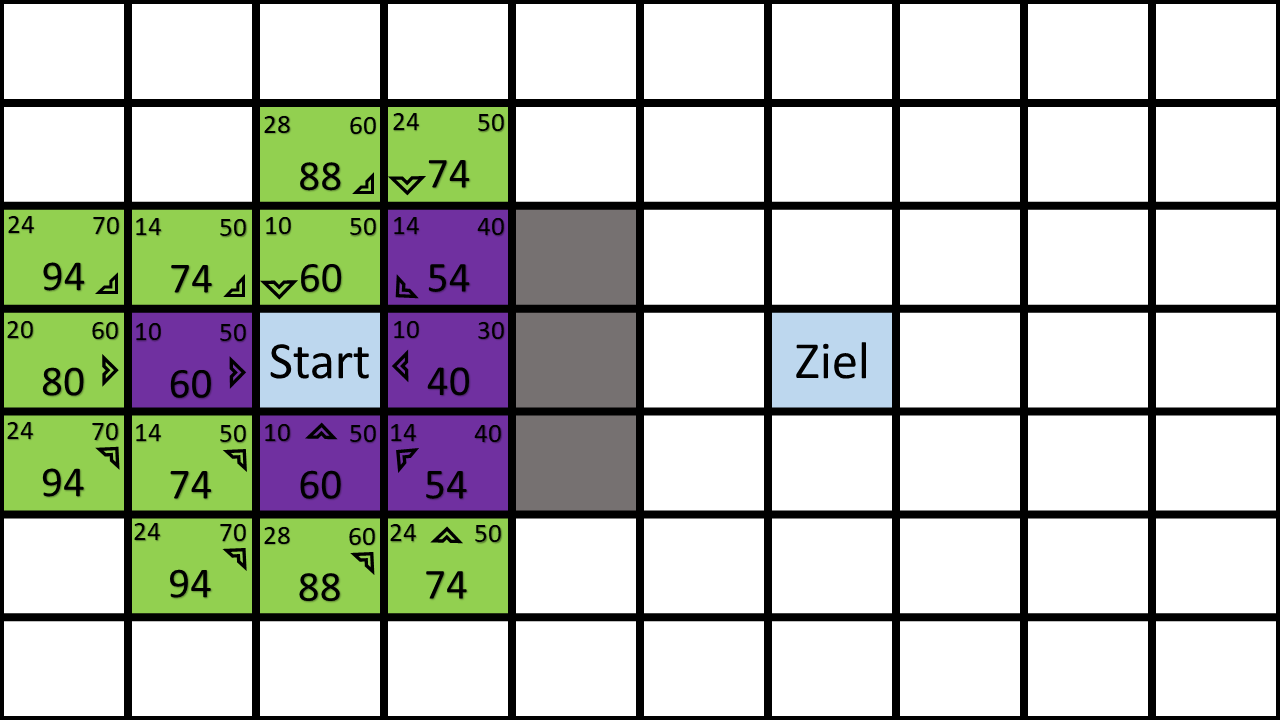
\includegraphics[width=\textwidth]{assets/aStarStep6.png}
        \caption{Schritt 7}
        \label{fig:aStartStep7}
    \end{subfigure}
    ~
    \begin{subfigure}[b]{0.3\textwidth}
        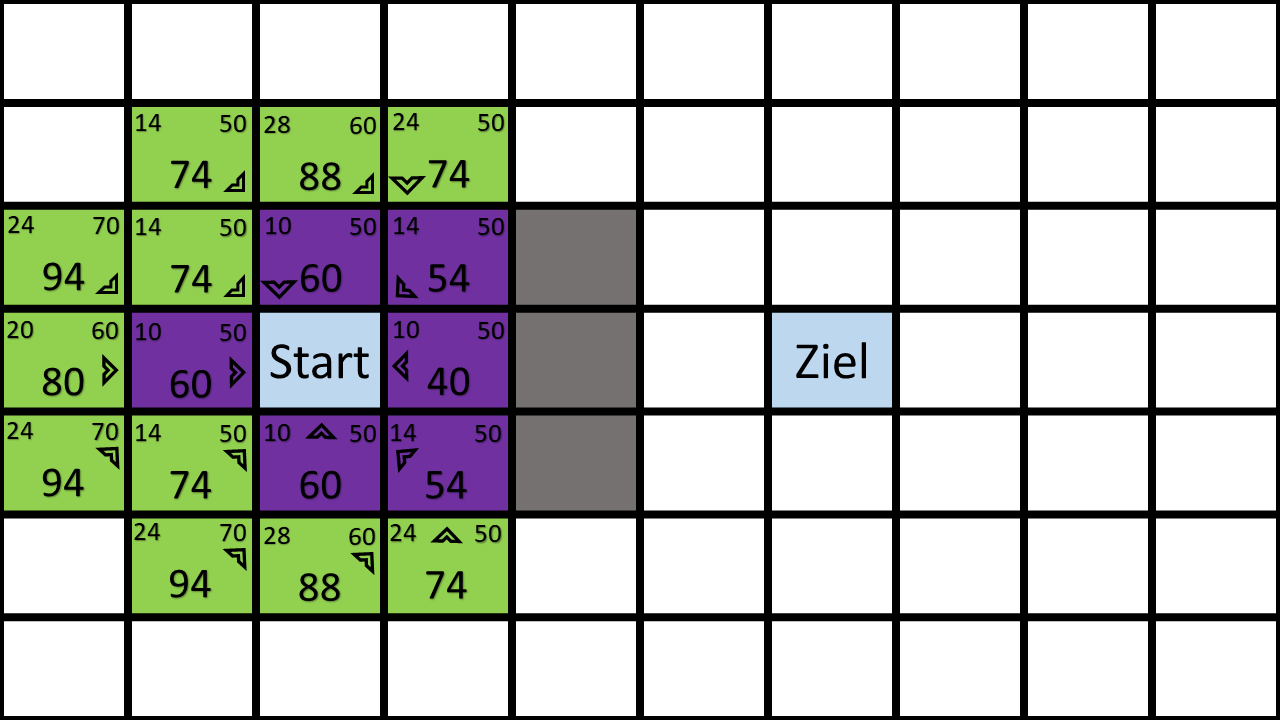
\includegraphics[width=\textwidth]{assets/aStarStep7.png}
        \caption{Schritt 8}
        \label{fig:aStartStep8}
    \end{subfigure}
    ~
    \begin{subfigure}[b]{0.3\textwidth}
        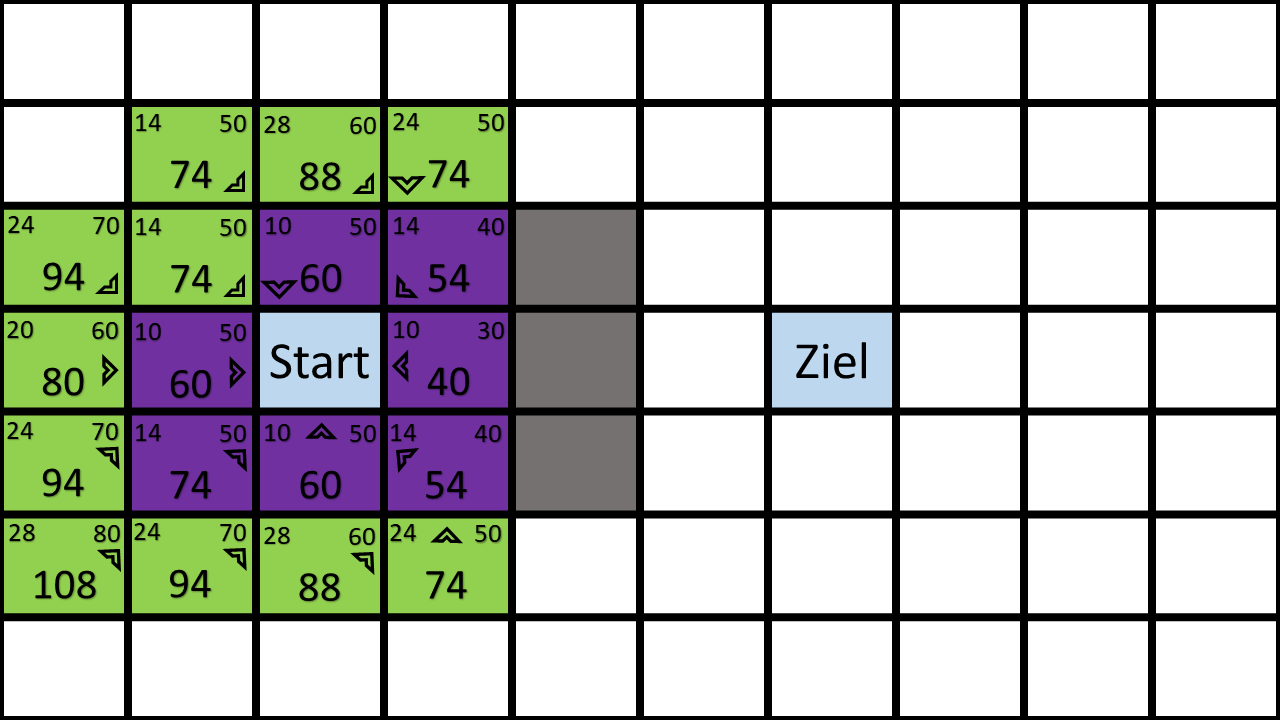
\includegraphics[width=\textwidth]{assets/aStarStep8.png}
        \caption{Schritt 9}
        \label{fig:aStartStep9}
    \end{subfigure}
    \caption{A* Ausführungsschritte 7-9}\label{fig:aStarStep7_9}
\end{figure}

\begin{figure}
    \centering
    \begin{subfigure}[b]{0.3\textwidth}
        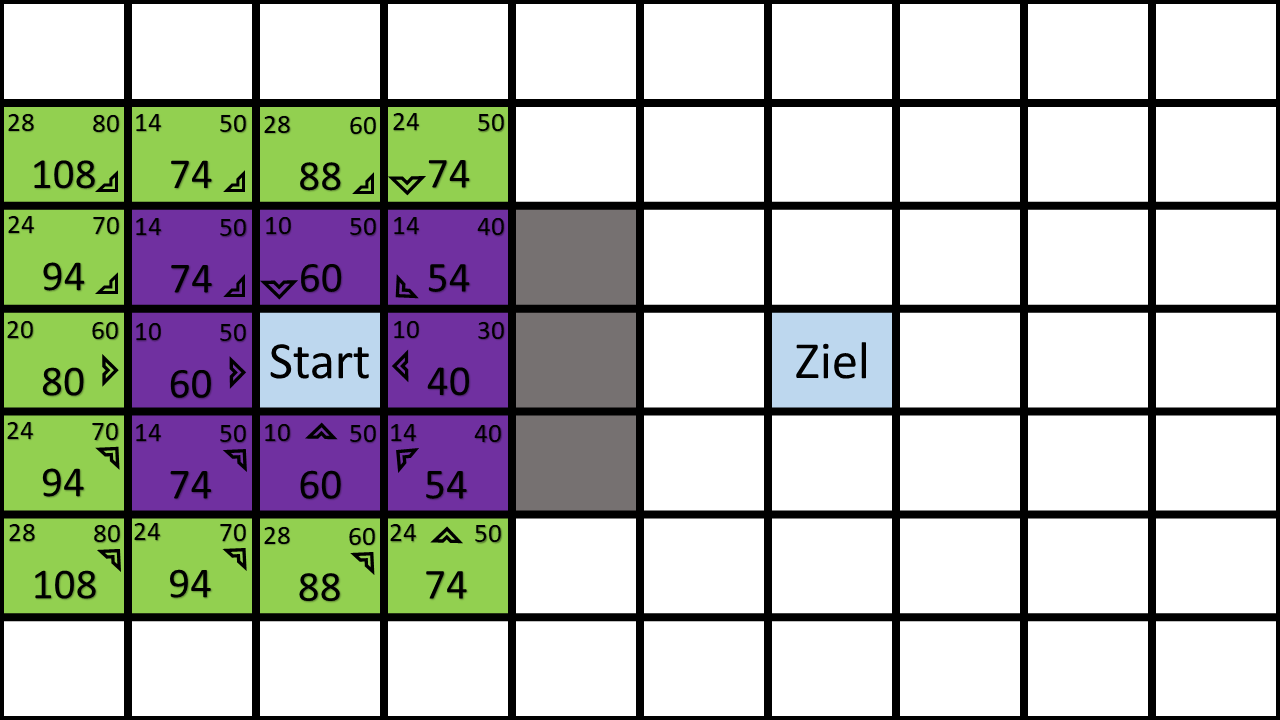
\includegraphics[width=\textwidth]{assets/aStarStep9.png}
        \caption{Schritt 10}
        \label{fig:aStartStep10}
    \end{subfigure}
    ~
    \begin{subfigure}[b]{0.3\textwidth}
        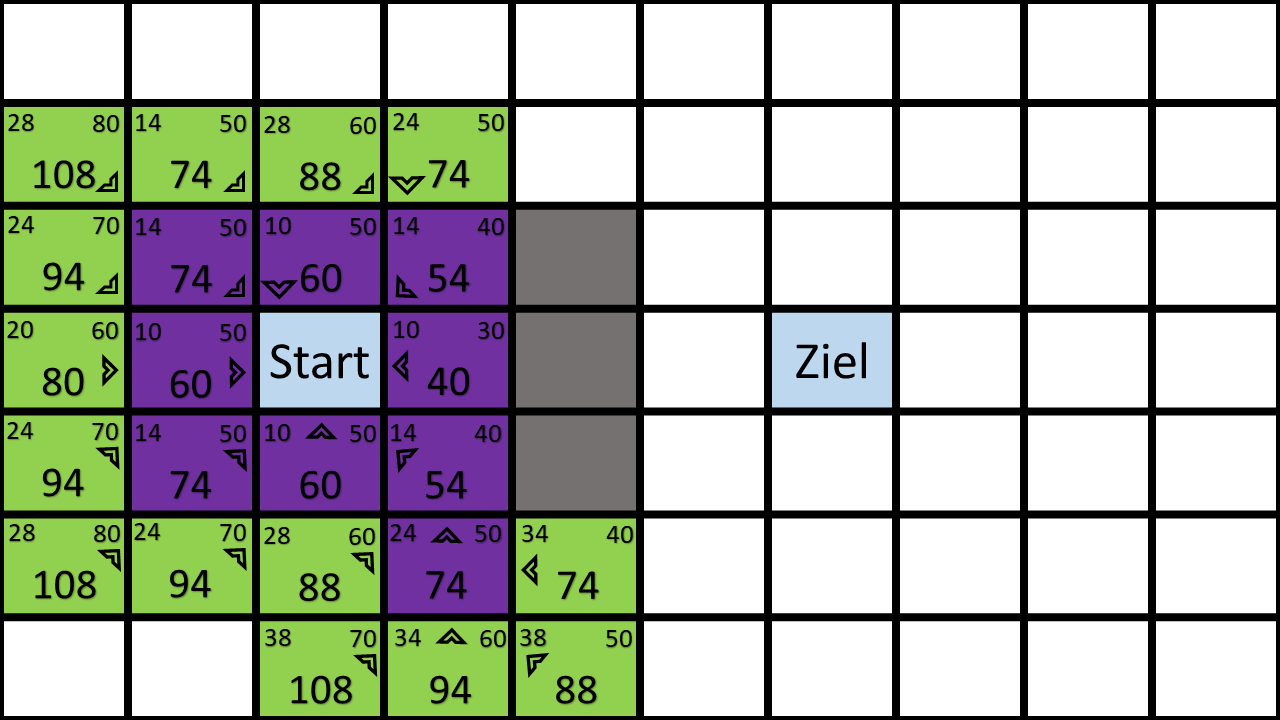
\includegraphics[width=\textwidth]{assets/aStarStep10.png}
        \caption{Schritt 11}
        \label{fig:aStartStep11}
    \end{subfigure}
    ~
    \begin{subfigure}[b]{0.3\textwidth}
        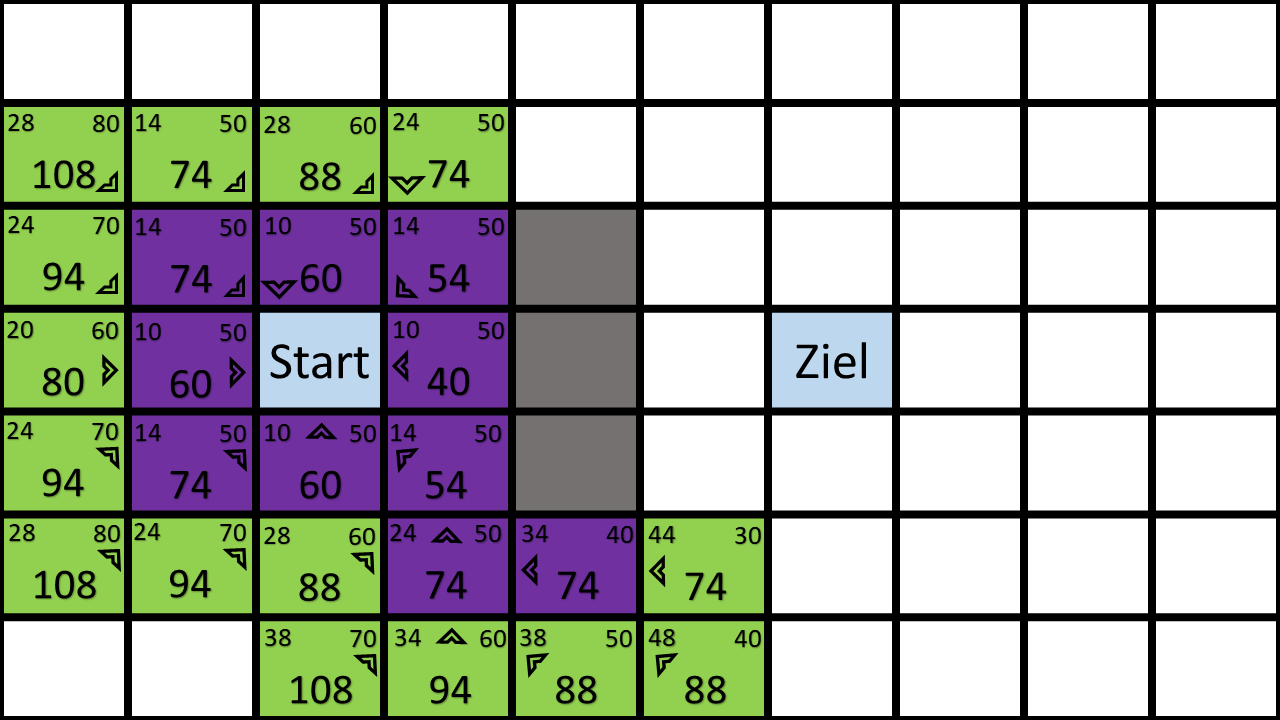
\includegraphics[width=\textwidth]{assets/aStarStep11.png}
        \caption{Schritt 12}
        \label{fig:aStartStep12}
    \end{subfigure}
    \caption{A* Ausführungsschritte 10-12}\label{fig:aStarStep10_12}
\end{figure}

\begin{figure}
    \centering
    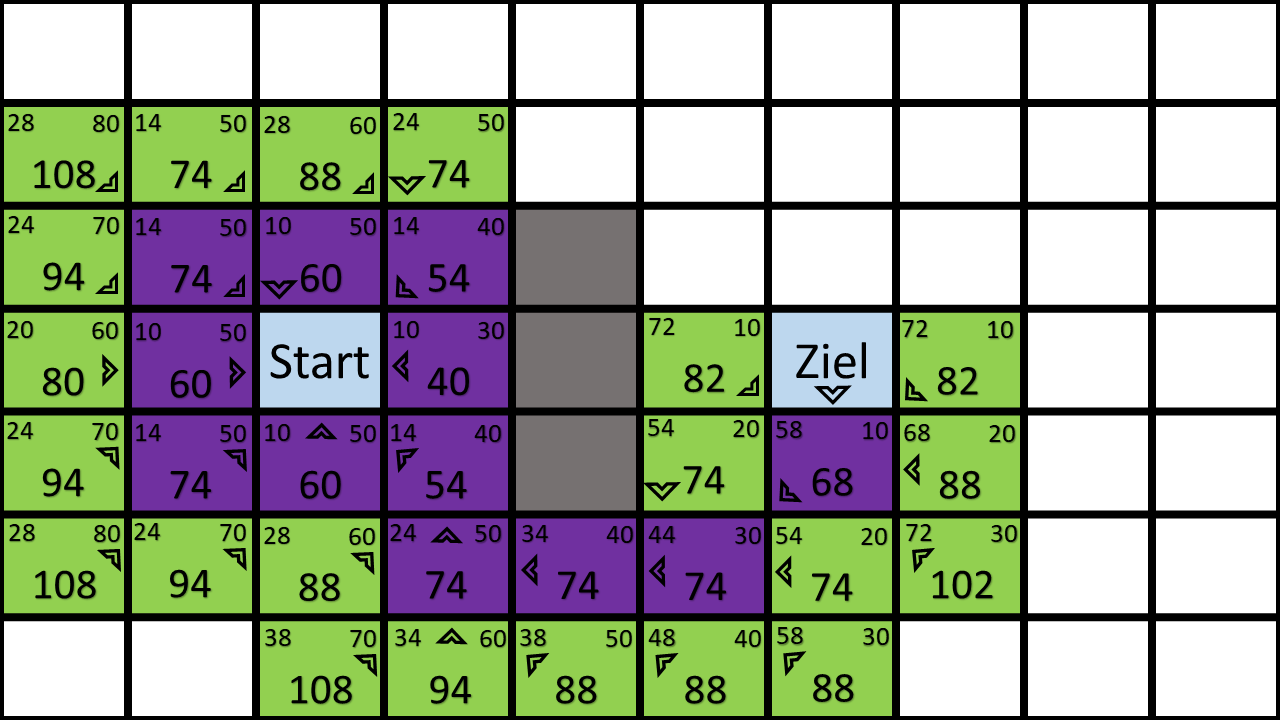
\includegraphics[width=\textwidth]{assets/aStarStep13.png}
    \caption{A* Schritt 13}\label{fig:aStarStep13}
\end{figure}

\label{sec:fundamentals}
\section{Unity}
Unity ist eine GameEngine die in diesem Projekt genutzt wird, um das Spiel zu entwickeln. Des Weiteren besteht Unity aus einem sehr umfangreichen Editor, mit dem ein Spieleentwickler eine große Auswahl an Tools zur Entwicklung erh\"alt. Unity bietet sowohl die M\"oglichkeit in 2D, als auch in 3D zu entwickeln.
